\documentclass[11pt,letterpaper]{article}

% Build steps (from this folder):
% 1) pdflatex Module3.tex
% 2) makeglossaries Module3
% 3) pdflatex Module3.tex
% 4) pdflatex Module3.tex

% ── Packages ──────────────────────────────────────────────────
\usepackage[margin=1in]{geometry}
\usepackage{titlesec}
\usepackage{enumitem}
\usepackage{booktabs}
\usepackage{tabularx}
\usepackage{graphicx}
\usepackage{xcolor}
\usepackage{hyperref}
\usepackage{fancyhdr}
\usepackage{amsmath}
\usepackage{amssymb}
\usepackage{tcolorbox}
\usepackage{multicol}
\usepackage{caption}
\usepackage{tikz}
\usepackage{listings}
\usepackage[acronym,toc,nopostdot]{glossaries}
\usetikzlibrary{shapes.geometric, arrows.meta, positioning, fit, calc, decorations.pathreplacing}
\makenoidxglossaries%
% Shared acronym macro container for EE800/820 lesson plan modules.
% Usage: type \IDE, \FPGA, \UART, etc. First use is expanded; later uses show acronym only.
% Requires in each document preamble:
%   \usepackage[acronym,toc]{glossaries}
%   \makeglossaries
%   % Shared acronym macro container for EE800/820 lesson plan modules.
% Usage: type \IDE, \FPGA, \UART, etc. First use is expanded; later uses show acronym only.
% Requires in each document preamble:
%   \usepackage[acronym,toc]{glossaries}
%   \makeglossaries
%   % Shared acronym macro container for EE800/820 lesson plan modules.
% Usage: type \IDE, \FPGA, \UART, etc. First use is expanded; later uses show acronym only.
% Requires in each document preamble:
%   \usepackage[acronym,toc]{glossaries}
%   \makeglossaries
%   \input{../glossary}
% Print used acronyms near end of document:
%   \printglossary[type=\acronymtype,title={Acronyms Used}]

% Acronym definitions (only used entries appear in the printed glossary).
\newacronym{ask}{ASK}{Amplitude Shift Keying}
\newacronym{bga}{BGA}{Ball Grid Array}
\newacronym{bom}{BOM}{Bill of Materials}
\newacronym{bram}{BRAM}{Block Random Access Memory}
\newacronym{crc}{CRC}{Cyclic Redundancy Check}
\newacronym{css}{CSS}{Chirp Spread Spectrum}
\newacronym{dma}{DMA}{Direct Memory Access}
\newacronym{dsp}{DSP}{Digital Signal Processing}
\newacronym{eda}{EDA}{Exploratory Data Analysis}
\newacronym{fifo}{FIFO}{First In, First Out}
\newacronym{fpga}{FPGA}{Field-Programmable Gate Array}
\newacronym{fsk}{FSK}{Frequency Shift Keying}
\newacronym{fsm}{FSM}{Finite State Machine}
\newacronym{gpio}{GPIO}{General-Purpose Input/Output}
\newacronym{hal}{HAL}{Hardware Abstraction Layer}
\newacronym{i2c}{I\textsuperscript{2}C}{Inter-Integrated Circuit}
\newacronym{ide}{IDE}{Integrated Development Environment}
\newacronym{ila}{ILA}{Integrated Logic Analyzer}
\newacronym{ism}{ISM}{Industrial, Scientific, and Medical}
\newacronym{isr}{ISR}{Interrupt Service Routine}
\newacronym{lut}{LUT}{Look-Up Table}
\newacronym{mcu}{MCU}{Microcontroller Unit}
\newacronym{ml}{ML}{Machine Learning}
\newacronym{ook}{OOK}{On-Off Keying}
\newacronym{per}{PER}{Packet Error Rate}
\newacronym{rf}{RF}{Radio Frequency}
\newacronym{rssi}{RSSI}{Received Signal Strength Indicator}
\newacronym{rtl}{RTL}{Register-Transfer Level}
\newacronym{snr}{SNR}{Signal-to-Noise Ratio}
\newacronym{spi}{SPI}{Serial Peripheral Interface}
\newacronym{uart}{UART}{Universal Asynchronous Receiver/Transmitter}
\newacronym{vhdl}{VHDL}{VHSIC Hardware Description Language}

% Convenience wrappers so you can type \IDE, \RF, etc.
\providecommand{\ASK}{\gls{ask}}
\providecommand{\BGA}{\gls{bga}}
\providecommand{\BOM}{\gls{bom}}
\providecommand{\BRAM}{\gls{bram}}
\providecommand{\CRC}{\gls{crc}}
\providecommand{\CSS}{\gls{css}}
\providecommand{\DMA}{\gls{dma}}
\providecommand{\DSP}{\gls{dsp}}
\providecommand{\EDA}{\gls{eda}}
\providecommand{\FIFO}{\gls{fifo}}
\providecommand{\FPGA}{\gls{fpga}}
\providecommand{\FSK}{\gls{fsk}}
\providecommand{\FSM}{\gls{fsm}}
\providecommand{\GPIO}{\gls{gpio}}
\providecommand{\HAL}{\gls{hal}}
\providecommand{\IIC}{\gls{i2c}}
\providecommand{\IDE}{\gls{ide}}
\providecommand{\ILA}{\gls{ila}}
\providecommand{\ISM}{\gls{ism}}
\providecommand{\ISR}{\gls{isr}}
\providecommand{\LUT}{\gls{lut}}
\providecommand{\MCU}{\gls{mcu}}
\providecommand{\ML}{\gls{ml}}
\providecommand{\OOK}{\gls{ook}}
\providecommand{\PER}{\gls{per}}
\providecommand{\RF}{\gls{rf}}
\providecommand{\RSSI}{\gls{rssi}}
\providecommand{\RTL}{\gls{rtl}}
\providecommand{\SNR}{\gls{snr}}
\providecommand{\SPI}{\gls{spi}}
\providecommand{\UART}{\gls{uart}}
\providecommand{\VHDL}{\gls{vhdl}}


% Print used acronyms near end of document:
%   \printglossary[type=\acronymtype,title={Acronyms Used}]

% Acronym definitions (only used entries appear in the printed glossary).
\newacronym{ask}{ASK}{Amplitude Shift Keying}
\newacronym{bga}{BGA}{Ball Grid Array}
\newacronym{bom}{BOM}{Bill of Materials}
\newacronym{bram}{BRAM}{Block Random Access Memory}
\newacronym{crc}{CRC}{Cyclic Redundancy Check}
\newacronym{css}{CSS}{Chirp Spread Spectrum}
\newacronym{dma}{DMA}{Direct Memory Access}
\newacronym{dsp}{DSP}{Digital Signal Processing}
\newacronym{eda}{EDA}{Exploratory Data Analysis}
\newacronym{fifo}{FIFO}{First In, First Out}
\newacronym{fpga}{FPGA}{Field-Programmable Gate Array}
\newacronym{fsk}{FSK}{Frequency Shift Keying}
\newacronym{fsm}{FSM}{Finite State Machine}
\newacronym{gpio}{GPIO}{General-Purpose Input/Output}
\newacronym{hal}{HAL}{Hardware Abstraction Layer}
\newacronym{i2c}{I\textsuperscript{2}C}{Inter-Integrated Circuit}
\newacronym{ide}{IDE}{Integrated Development Environment}
\newacronym{ila}{ILA}{Integrated Logic Analyzer}
\newacronym{ism}{ISM}{Industrial, Scientific, and Medical}
\newacronym{isr}{ISR}{Interrupt Service Routine}
\newacronym{lut}{LUT}{Look-Up Table}
\newacronym{mcu}{MCU}{Microcontroller Unit}
\newacronym{ml}{ML}{Machine Learning}
\newacronym{ook}{OOK}{On-Off Keying}
\newacronym{per}{PER}{Packet Error Rate}
\newacronym{rf}{RF}{Radio Frequency}
\newacronym{rssi}{RSSI}{Received Signal Strength Indicator}
\newacronym{rtl}{RTL}{Register-Transfer Level}
\newacronym{snr}{SNR}{Signal-to-Noise Ratio}
\newacronym{spi}{SPI}{Serial Peripheral Interface}
\newacronym{uart}{UART}{Universal Asynchronous Receiver/Transmitter}
\newacronym{vhdl}{VHDL}{VHSIC Hardware Description Language}

% Convenience wrappers so you can type \IDE, \RF, etc.
\providecommand{\ASK}{\gls{ask}}
\providecommand{\BGA}{\gls{bga}}
\providecommand{\BOM}{\gls{bom}}
\providecommand{\BRAM}{\gls{bram}}
\providecommand{\CRC}{\gls{crc}}
\providecommand{\CSS}{\gls{css}}
\providecommand{\DMA}{\gls{dma}}
\providecommand{\DSP}{\gls{dsp}}
\providecommand{\EDA}{\gls{eda}}
\providecommand{\FIFO}{\gls{fifo}}
\providecommand{\FPGA}{\gls{fpga}}
\providecommand{\FSK}{\gls{fsk}}
\providecommand{\FSM}{\gls{fsm}}
\providecommand{\GPIO}{\gls{gpio}}
\providecommand{\HAL}{\gls{hal}}
\providecommand{\IIC}{\gls{i2c}}
\providecommand{\IDE}{\gls{ide}}
\providecommand{\ILA}{\gls{ila}}
\providecommand{\ISM}{\gls{ism}}
\providecommand{\ISR}{\gls{isr}}
\providecommand{\LUT}{\gls{lut}}
\providecommand{\MCU}{\gls{mcu}}
\providecommand{\ML}{\gls{ml}}
\providecommand{\OOK}{\gls{ook}}
\providecommand{\PER}{\gls{per}}
\providecommand{\RF}{\gls{rf}}
\providecommand{\RSSI}{\gls{rssi}}
\providecommand{\RTL}{\gls{rtl}}
\providecommand{\SNR}{\gls{snr}}
\providecommand{\SPI}{\gls{spi}}
\providecommand{\UART}{\gls{uart}}
\providecommand{\VHDL}{\gls{vhdl}}


% Print used acronyms near end of document:
%   \printglossary[type=\acronymtype,title={Acronyms Used}]

% Acronym definitions (only used entries appear in the printed glossary).
\newacronym{ask}{ASK}{Amplitude Shift Keying}
\newacronym{bga}{BGA}{Ball Grid Array}
\newacronym{bom}{BOM}{Bill of Materials}
\newacronym{bram}{BRAM}{Block Random Access Memory}
\newacronym{crc}{CRC}{Cyclic Redundancy Check}
\newacronym{css}{CSS}{Chirp Spread Spectrum}
\newacronym{dma}{DMA}{Direct Memory Access}
\newacronym{dsp}{DSP}{Digital Signal Processing}
\newacronym{eda}{EDA}{Exploratory Data Analysis}
\newacronym{fifo}{FIFO}{First In, First Out}
\newacronym{fpga}{FPGA}{Field-Programmable Gate Array}
\newacronym{fsk}{FSK}{Frequency Shift Keying}
\newacronym{fsm}{FSM}{Finite State Machine}
\newacronym{gpio}{GPIO}{General-Purpose Input/Output}
\newacronym{hal}{HAL}{Hardware Abstraction Layer}
\newacronym{i2c}{I\textsuperscript{2}C}{Inter-Integrated Circuit}
\newacronym{ide}{IDE}{Integrated Development Environment}
\newacronym{ila}{ILA}{Integrated Logic Analyzer}
\newacronym{ism}{ISM}{Industrial, Scientific, and Medical}
\newacronym{isr}{ISR}{Interrupt Service Routine}
\newacronym{lut}{LUT}{Look-Up Table}
\newacronym{mcu}{MCU}{Microcontroller Unit}
\newacronym{ml}{ML}{Machine Learning}
\newacronym{ook}{OOK}{On-Off Keying}
\newacronym{per}{PER}{Packet Error Rate}
\newacronym{rf}{RF}{Radio Frequency}
\newacronym{rssi}{RSSI}{Received Signal Strength Indicator}
\newacronym{rtl}{RTL}{Register-Transfer Level}
\newacronym{snr}{SNR}{Signal-to-Noise Ratio}
\newacronym{spi}{SPI}{Serial Peripheral Interface}
\newacronym{uart}{UART}{Universal Asynchronous Receiver/Transmitter}
\newacronym{vhdl}{VHDL}{VHSIC Hardware Description Language}

% Convenience wrappers so you can type \IDE, \RF, etc.
\providecommand{\ASK}{\gls{ask}}
\providecommand{\BGA}{\gls{bga}}
\providecommand{\BOM}{\gls{bom}}
\providecommand{\BRAM}{\gls{bram}}
\providecommand{\CRC}{\gls{crc}}
\providecommand{\CSS}{\gls{css}}
\providecommand{\DMA}{\gls{dma}}
\providecommand{\DSP}{\gls{dsp}}
\providecommand{\EDA}{\gls{eda}}
\providecommand{\FIFO}{\gls{fifo}}
\providecommand{\FPGA}{\gls{fpga}}
\providecommand{\FSK}{\gls{fsk}}
\providecommand{\FSM}{\gls{fsm}}
\providecommand{\GPIO}{\gls{gpio}}
\providecommand{\HAL}{\gls{hal}}
\providecommand{\IIC}{\gls{i2c}}
\providecommand{\IDE}{\gls{ide}}
\providecommand{\ILA}{\gls{ila}}
\providecommand{\ISM}{\gls{ism}}
\providecommand{\ISR}{\gls{isr}}
\providecommand{\LUT}{\gls{lut}}
\providecommand{\MCU}{\gls{mcu}}
\providecommand{\ML}{\gls{ml}}
\providecommand{\OOK}{\gls{ook}}
\providecommand{\PER}{\gls{per}}
\providecommand{\RF}{\gls{rf}}
\providecommand{\RSSI}{\gls{rssi}}
\providecommand{\RTL}{\gls{rtl}}
\providecommand{\SNR}{\gls{snr}}
\providecommand{\SPI}{\gls{spi}}
\providecommand{\UART}{\gls{uart}}
\providecommand{\VHDL}{\gls{vhdl}}



% ── Colors ────────────────────────────────────────────────────
\definecolor{stevens}{RGB}{163,31,52}       % Stevens Red
\definecolor{darkgray}{RGB}{60,60,60}
\definecolor{lightgray}{RGB}{240,240,240}
\definecolor{accentblue}{RGB}{30,80,140}

% ── Hyperref Setup ────────────────────────────────────────────
\hypersetup{
	colorlinks=true,
	linkcolor=stevens,
	urlcolor=accentblue,
	citecolor=darkgray,
	plainpages=false
}

% ── Header / Footer ──────────────────────────────────────────
\pagestyle{fancy}
\fancyhf{}
\fancyhead[L]{\small\textcolor{darkgray}{Stevens Institute of Technology}}
\fancyhead[R]{\small\textcolor{darkgray}{Spring 2026}}
\fancyfoot[C]{\thepage}
\renewcommand{\headrulewidth}{0.4pt}

% ── Section Formatting ───────────────────────────────────────
\titleformat{\section}
{\Large\bfseries\color{stevens}}{\thesection}{1em}{}[\vspace{-0.5em}\rule{\textwidth}{0.4pt}]
\titleformat{\subsection}
{\large\bfseries\color{darkgray}}{\thesubsection}{1em}{}

% ── tcolorbox Styles ─────────────────────────────────────────
\tcbset{
	objective/.style={colback=lightgray, colframe=stevens,
		fonttitle=\bfseries, title=#1, boxrule=0.5pt, arc=2pt},
	infobox/.style={colback=blue!5, colframe=accentblue,
		fonttitle=\bfseries, title=#1, boxrule=0.5pt, arc=2pt},
	deliverable/.style={colback=green!5, colframe=green!40!black,
		fonttitle=\bfseries, title=#1, boxrule=0.5pt, arc=2pt},
	warning/.style={colback=red!5, colframe=stevens,
		fonttitle=\bfseries, title=#1, boxrule=0.5pt, arc=2pt}
}

% ── Listings Style ───────────────────────────────────────────
\lstset{
	basicstyle=\small\ttfamily,
	keywordstyle=\color{accentblue}\bfseries,
	commentstyle=\color{darkgray}\itshape,
	stringstyle=\color{stevens},
	numbers=left,
	numberstyle=\tiny\color{darkgray},
	numbersep=8pt,
	frame=single,
	framerule=0.4pt,
	rulecolor=\color{darkgray},
	backgroundcolor=\color{lightgray},
	breaklines=true,
	tabsize=2,
	showstringspaces=false,
	captionpos=b
}

% ══════════════════════════════════════════════════════════════
\begin{document}

	% ── Title Page ───────────────────────────────────────────────
	\pagenumbering{Alph}
	\begin{titlepage}
		\centering
		\vspace*{2cm}

		{\Huge\bfseries\color{stevens} Lesson Plan: Module~3\par}
		\vspace{0.5cm}
		{\LARGE\color{darkgray} System Integration, End-to-End Verification,\\[4pt]
			and Structured Data Collection\par}

		\vspace{1.5cm}
		\rule{0.6\textwidth}{1pt}
		\vspace{1.5cm}

		{\Large\textbf{An Educational Framework for\\[4pt]
				AI-Driven Signal Processing}\par}

		\vspace{1.5cm}

		\begin{tabular}{rl}
			\textbf{Student:}         & Jude Eschete \\
			\textbf{Project Advisor:} & Dr.\ Bernard Yett \\
			\textbf{Program:}         & M.S.\ Computer Engineering \\
			\textbf{Institution:}     & Stevens Institute of Technology \\
			\textbf{Date Range:}      & March 29 -- April 11, 2026 \\
		\end{tabular}

		\vspace{2cm}

		\begin{tcolorbox}[colback=lightgray, colframe=darkgray, width=0.85\textwidth, arc=2pt]
			\centering\small
			This document presents the lesson plan for the third module of the capstone project.
			Students connect the STM32 beacon--receiver subsystem (Module~1) with the Field-Programmable Gate Array signal
			processing pipeline (Module~2), diagnose and resolve integration failures that surface
			when individually tested subsystems operate together on real hardware, characterize
			end-to-end latency and throughput, and execute structured data collection campaigns
			that produce the labeled Radio Frequency dataset for the Machine Learning pipeline in Module~4.
		\end{tcolorbox}

		\vfill
		{\small\textcolor{darkgray}{JEschete@stevens.edu}}
	\end{titlepage}

	% ── Table of Contents ────────────────────────────────────────
	\pagenumbering{roman}
	\tableofcontents
	\newpage
	\pagenumbering{arabic}

	% ══════════════════════════════════════════════════════════════
	\section{Module Overview}
	% ══════════════════════════════════════════════════════════════

	\begin{tcolorbox}[objective={Module 3 Learning Objectives}]
		Upon completion of this module, the student (or future learner following this curriculum) will be able to:
		\begin{enumerate}[label=\textbf{LO-\arabic*}]
			\item Deploy the Module~2 \FPGA{} bitstream to the Nexys A7-100T and verify correct operation against live \UART{} data from the STM32 receiver, identifying and resolving discrepancies between simulation behavior and hardware behavior.
			\item Diagnose integration failures that span disciplinary boundaries---firmware timing errors that corrupt the \FPGA{} data stream, baud rate drift, impedance mismatches, and protocol synchronization faults---using systematic debugging techniques (\ILA{} probes, logic analyzer captures, \UART{} logging).
			\item Measure and characterize end-to-end system performance metrics: \PER{}, end-to-end latency (beacon TX to feature vector availability), sustained throughput, and \FIFO{} utilization under load.
			\item Design and execute a structured data collection campaign that systematically varies beacon parameters (TX power, spreading factor, modulation type, number of concurrent beacons, physical distance) to produce a labeled \RF{} dataset with controlled experimental conditions.
			\item Implement a host-side Python data collection script that receives feature vectors from the \FPGA{}, attaches ground-truth labels, and stores the dataset in a format ready for machine learning ingestion.
			\item Identify and articulate the distribution shift between simulation data and hardware-collected data, understanding how real-world channel impairments, timing offsets, and hardware non-idealities produce feature distributions that differ from idealized models.
		\end{enumerate}
	\end{tcolorbox}

	\subsection{Context Within the Project}

	Module~3 represents the critical integration point of the curriculum. Modules~1 and~2 each developed and validated subsystems in isolation: Module~1 produced a working beacon--receiver \RF{} subsystem with known packet formats and timing; Module~2 produced a simulated-and-verified \FPGA{} ingestion pipeline that parses those packets and extracts feature vectors. Neither module tested whether these subsystems work correctly when connected to each other through a physical interface carrying real signals.

	This gap is intentional. The framework's central pedagogical thesis is that cross-domain integration failures are the primary subject of instruction, not incidental obstacles. A firmware direct memory access (\DMA{}) timing error that has no observable effect during Module~1 standalone testing may cause byte-level misalignment in the \FPGA{} parser. A \CRC{} engine that passes every simulation testbench in Module~2 may reject valid frames on hardware due to a byte-ordering mismatch in the STM32 firmware. These failures require students to reason simultaneously across firmware, hardware interface, and digital logic domains---the exact multidisciplinary skill the framework is designed to develop.

	The second half of this module shifts from integration debugging to structured data collection. The validated end-to-end pipeline becomes a scientific instrument: students use it to execute controlled experiments that vary beacon parameters and collect the labeled \RF{} feature dataset that drives all machine learning work in Module~4. The quality, diversity, and labeling integrity of this dataset directly determine what classifiers can be trained and how well they generalize. This dependency makes the data collection campaign a non-trivial engineering exercise, not merely a ``run the system and save files'' activity.

	\subsection{Prerequisites}

	Students beginning this module should have:
	\begin{itemize}[leftmargin=2em]
		\item Completed Module~1 with a working multi-beacon \RF{} subsystem (at least 2 beacons + 1 receiver, all validated for packet transmission and reception).
		\item Completed Module~2 with a fully simulated \FPGA{} pipeline (\UART{} RX $\rightarrow$ parser $\rightarrow$ \CRC{} $\rightarrow$ feature extraction $\rightarrow$ block random access memory (\BRAM{})), a generated bitstream, and a verified constraint file (\texttt{.xdc}).
		\item All hardware assembled and wired: STM32 receiver \UART{} TX connected to Nexys A7 PMOD JA, \FPGA{} USB-\UART{} connected to host PC, beacons powered and antennas attached.
		\item Python~3.10+ with \texttt{pyserial} installed on the host machine.
		\item Familiarity with Vivado \ILA{} (Integrated Logic Analyzer) for on-chip signal probing.
		\item Access to a logic analyzer (optional but recommended for Week~1 debugging).
	\end{itemize}

	\newpage
	% ══════════════════════════════════════════════════════════════
	\section{Weekly Schedule}
	% ══════════════════════════════════════════════════════════════

	The module spans two weeks (four working sessions). The first week focuses on hardware deployment, integration debugging, and performance characterization. The second week focuses on structured data collection and dataset preparation.

	\begin{table}[ht!]
		\centering
		\caption{Module 3 weekly breakdown.}
		\label{tab:schedule}
		\renewcommand{\arraystretch}{1.4}
		\begin{tabularx}{\textwidth}{c l X}
			\toprule
			\textbf{Week} & \textbf{Focus Area} & \textbf{Key Activities} \\
			\midrule
			1 & Hardware Deployment \& Integration Debugging &
			Program \FPGA{} with Module~2 bitstream; connect STM32 receiver; diagnose and resolve integration failures (baud mismatch, byte alignment, \CRC{} rejects); verify first live frame through the complete pipeline. \\
			2 & Performance Characterization &
			Measure end-to-end latency, throughput, and packet error rate; stress-test with multiple beacons; identify bottlenecks; tune \FIFO{} depths and export timing; document system performance envelope. \\
			3 & Data Collection Campaign Design \& Execution &
			Design experimental matrix (TX power, SF, modulation, distance, beacon count); implement host-side Python collection script; execute single-variable sweep campaigns; validate dataset integrity and label correctness. \\
			4 & Multi-Variable Collection \& Dataset Finalization &
			Execute multi-variable and edge-case collection runs; merge and clean dataset; perform exploratory data analysis; document dataset structure, provenance, and known limitations for Module~4 handoff. \\
			\bottomrule
		\end{tabularx}
	\end{table}

	\newpage
	% ══════════════════════════════════════════════════════════════
	\section{Week 1: Hardware Deployment and Integration Debugging}
	\label{sec:integration}
	% ══════════════════════════════════════════════════════════════

	\subsection{Objectives}

	\begin{itemize}[leftmargin=2em]
		\item Program the Nexys A7-100T with the Module~2 bitstream and verify basic I/O (LEDs, pushbuttons, seven-segment display).
		\item Connect the STM32 receiver's \UART{} TX to the \FPGA{}'s PMOD input and observe the first live data on the \FPGA{}.
		\item Diagnose and resolve integration failures using a systematic debugging methodology.
		\item Achieve the first successfully parsed and \CRC{}-verified frame on live hardware.
	\end{itemize}

	\subsection{Deployment Checklist}

	Before connecting subsystems, each component must be verified independently on the bench:

	\begin{table}[ht!]
		\centering
		\caption{Pre-integration hardware checklist.}
		\label{tab:checklist}
		\renewcommand{\arraystretch}{1.3}
		\begin{tabularx}{\textwidth}{c X c}
			\toprule
			\textbf{\#} & \textbf{Check} & \textbf{Pass?} \\
			\midrule
			1 & Nexys A7 powers on via USB; Vivado Hardware Manager detects the \FPGA{}. & $\square$ \\
			2 & Module~2 bitstream programs successfully; LED test pattern confirms I/O. & $\square$ \\
			3 & \FPGA{} USB-\UART{} loopback: characters typed in terminal echo back correctly at 115200 baud. & $\square$ \\
			4 & STM32 receiver firmware loaded; beacon packets print to STM32 debug \UART{}. & $\square$ \\
			5 & Beacon~A transmitting (LED blink or debug \UART{} confirms TX cycle). & $\square$ \\
			6 & Beacon~B transmitting (same verification). & $\square$ \\
			7 & Receiver reports both beacon IDs in debug log with valid \RSSI{}/\SNR{}. & $\square$ \\
			8 & Physical wiring: receiver \UART{} TX $\rightarrow$ PMOD JA pin~1; GND connected between boards. & $\square$ \\
			\bottomrule
		\end{tabularx}
	\end{table}

	\begin{tcolorbox}[warning={Critical: Common Ground}]
		The STM32 Nucleo and Nexys A7 are powered from separate USB ports and therefore have separate ground references. A dedicated GND jumper wire between the Nucleo GND pin and the PMOD JA GND pin is \textbf{mandatory}. Without a common ground, the \UART{} signal levels are referenced to different potentials and the \FPGA{} will read garbage. This is the single most common integration failure in multi-board \UART{} connections and is trivially fixed but surprisingly easy to overlook.
	\end{tcolorbox}

	\subsection{Integration Debugging Methodology}

	Integration failures fall into predictable categories. The following systematic approach isolates the root cause efficiently:

	\subsubsection{Layer 1: Physical Interface}

	\begin{itemize}[leftmargin=2em]
		\item \textbf{Symptom:} \FPGA{} sees no transitions on \texttt{uart\_rxd}; LED frame counter stays at zero.
		\item \textbf{Diagnosis:} Probe the PMOD pin with an oscilloscope or logic analyzer. If no activity is visible, the wiring or pin assignment is wrong. Verify the STM32 TX pin mapping, the PMOD pin number, and the \texttt{.xdc} constraint file entry.
		\item \textbf{Common causes:} TX/RX swap (receiver TX connected to wrong PMOD pin); missing GND jumper; PMOD pin constrained to wrong \FPGA{} ball in \texttt{.xdc}; STM32 \UART{} TX not configured on the expected \GPIO{}.
	\end{itemize}

	\subsubsection{Layer 2: Baud Rate and Framing}

	\begin{itemize}[leftmargin=2em]
		\item \textbf{Symptom:} \FPGA{} sees transitions but \texttt{rx\_error} (framing error) asserts frequently; parsed bytes are incorrect.
		\item \textbf{Diagnosis:} Use a logic analyzer to capture the \UART{} waveform and manually verify the bit timing. Measure the actual bit period and compare to the expected 8.68~$\mu$s. Calculate the baud rate deviation.

		\begin{equation}
			\text{Deviation (\%)} = \frac{|T_{\text{measured}} - T_{\text{expected}}|}{T_{\text{expected}}} \times 100
			\label{eq:baud_deviation}
		\end{equation}

		The Module~2 \UART{} receiver tolerates $\pm 3\%$ with $16\times$ oversampling. If the deviation exceeds this, the STM32's baud rate prescaler must be adjusted.

		\item \textbf{Common causes:} STM32 system clock misconfigured (e.g., running at 72~MHz instead of 80~MHz, producing a different \UART{} divisor); \FPGA{} baud rate generic set incorrectly; stop bit configuration mismatch (STM32 sending 2 stop bits, \FPGA{} expecting 1).
	\end{itemize}

	\subsubsection{Layer 3: Protocol Synchronization}

	\begin{itemize}[leftmargin=2em]
		\item \textbf{Symptom:} Bytes arrive correctly (no framing errors) but the parser never asserts \texttt{frame\_valid}; it remains stuck in HUNT state.
		\item \textbf{Diagnosis:} Use the Vivado \ILA{} to capture the byte stream entering the parser. Look for the \texttt{0x7E} start delimiter. If it never appears, the receiver firmware may not be emitting the framing format expected by the parser (e.g., sending raw beacon packets without the receiver forwarding frame wrapper defined in Module~1 Table~6).
		\item \textbf{Common causes:} Receiver firmware updated since Module~1 with a different frame format; start delimiter value changed; STM32 byte ordering (endianness) differs from \FPGA{} expectation.
	\end{itemize}

	\subsubsection{Layer 4: Data Integrity}

	\begin{itemize}[leftmargin=2em]
		\item \textbf{Symptom:} Parser finds \texttt{0x7E} and progresses through states, but \CRC{}-8 rejects every frame.
		\item \textbf{Diagnosis:} Capture the complete 43-byte frame in the \ILA{}. Manually compute the \CRC{}-8 over bytes 1--41 and compare to byte~42. If the manual \CRC{} matches byte~42 but the hardware \CRC{} does not, the \VHDL{} \CRC{} implementation has a bug (likely initialization or byte-ordering). If the manual \CRC{} does \emph{not} match byte~42, the STM32 firmware is computing the \CRC{} differently (different polynomial, different initialization, or different byte range).
		\item \textbf{Common causes:} \CRC{} polynomial mismatch between firmware and \RTL{}; \CRC{} initialization value mismatch; firmware includes the start delimiter in the \CRC{} computation but the \RTL{} does not (or vice versa); endianness disagreement on multi-byte fields.
	\end{itemize}

	\begin{tcolorbox}[infobox={Design Principle: Integration Failures Are Learning Objectives}]
		The debugging categories above are not a list of mistakes to avoid---they are the \emph{subject matter} of this module. Each failure mode requires the student to reason across the firmware/hardware boundary and understand how a decision in one domain (e.g., the STM32's \CRC{} initialization value) propagates requirements into another domain (the \VHDL{} \CRC{} module). The framework deliberately stages development so that these mismatches are likely to occur: Module~1 and Module~2 are developed in partial isolation precisely so that integration surfaces real cross-domain issues. A curriculum that pre-solves these mismatches would eliminate the most valuable learning experiences.
	\end{tcolorbox}

	\subsection{Vivado Integrated Logic Analyzer (\ILA{})}

	The \ILA{} is the primary on-chip debugging tool for \FPGA{} integration. It captures internal signal transitions into block RAM and streams the captured data to Vivado's waveform viewer over JTAG.

	\subsubsection{Recommended \ILA{} Probe Points}

	\begin{table}[ht!]
		\centering
		\caption{\ILA{} probe signals for integration debugging.}
		\label{tab:ila}
		\renewcommand{\arraystretch}{1.3}
		\begin{tabularx}{\textwidth}{l c X}
			\toprule
			\textbf{Signal} & \textbf{Width} & \textbf{Purpose} \\
			\midrule
			\texttt{uart\_rxd} (synchronized) & 1 & Verify serial transitions are reaching \FPGA{} \\
			\texttt{rx\_data[7:0]} & 8 & Decoded bytes from \UART{} receiver \\
			\texttt{rx\_valid} & 1 & Byte-level timing; verify one pulse per byte \\
			\texttt{rx\_error} & 1 & Framing error detection \\
			\texttt{parser\_state[2:0]} & 3 & Parser \FSM{} state (HUNT, LENGTH, META, etc.) \\
			\texttt{byte\_counter[5:0]} & 6 & Position within current frame \\
			\texttt{frame\_valid} & 1 & Trigger: successful frame reception \\
			\texttt{frame\_reject} & 1 & Trigger: \CRC{} failure \\
			\texttt{beacon\_id[7:0]} & 8 & Parsed beacon ID (verify correct extraction) \\
			\texttt{rssi[7:0]} & 8 & Parsed \RSSI{} (compare to STM32 debug log) \\
			\texttt{fifo\_count[5:0]} & 6 & \FIFO{} occupancy (detect overflow risk) \\
			\bottomrule
		\end{tabularx}
	\end{table}

	\begin{tcolorbox}[warning={\ILA{} Resource Cost}]
		Each \ILA{} probe consumes block RAM for the capture buffer. A typical configuration---12 probes, 1024-sample depth---uses approximately 4 \BRAM{} tiles. This is acceptable during integration debugging (the Module~2 pipeline uses only 5 of 270 available \BRAM{} tiles) but should be removed from the final production bitstream to free resources. Mark \ILA{} instantiations with a generate conditional controlled by a top-level generic (\texttt{g\_DEBUG : boolean := true}) so they can be excluded without editing \RTL{}.
	\end{tcolorbox}

	\subsection{First Live Frame Verification}

	\begin{tcolorbox}[infobox={Exercise: First Frame on Hardware}]
		With one beacon transmitting at 2-second intervals and the receiver connected to the \FPGA{}:
		\begin{enumerate}
			\item Program the \FPGA{} and open the \ILA{} dashboard in Vivado.
			\item Set the \ILA{} trigger to \texttt{frame\_valid} rising edge.
			\item Arm the trigger and wait for a capture.
			\item When a frame is captured, verify the following against the STM32 receiver debug log:
			\begin{itemize}
				\item The parsed Beacon ID matches the transmitting beacon's configured ID.
				\item The parsed \RSSI{} is within $\pm 2$~dB of the value reported by the STM32.
				\item The sequence number matches the beacon's current count.
				\item Both \CRC{} checks pass (\texttt{frame\_valid} = `1', \texttt{beacon\_crc\_ok} = `1').
			\end{itemize}
			\item If the trigger never fires (no \texttt{frame\_valid}), set the trigger to \texttt{rx\_valid} rising edge instead and verify that bytes are arriving. Work through the debugging layers above.
		\end{enumerate}
		\textbf{Milestone:} The first successfully parsed live frame represents a validated end-to-end data path spanning all four hardware components (beacon \MCU{} $\rightarrow$ \RF{} link $\rightarrow$ receiver \MCU{} $\rightarrow$ \FPGA{} fabric).
	\end{tcolorbox}

	\begin{tcolorbox}[deliverable={Week 1 Deliverable}]
		\textbf{Integration Debug Report} --- A document containing:
		\begin{enumerate}
			\item Pre-integration checklist results (Table~\ref{tab:checklist}), with photos of the physical setup.
			\item Log of all integration issues encountered, categorized by debugging layer (physical, baud rate, protocol, data integrity), with root cause and resolution for each.
			\item \ILA{} waveform captures showing: first successful frame reception, parser state transitions during a live frame, and at least one diagnosed failure (before the fix was applied).
			\item Side-by-side comparison of \FPGA{}-parsed field values vs.\ STM32 debug log values for 10 consecutive frames.
		\end{enumerate}
	\end{tcolorbox}

	\newpage
	% ══════════════════════════════════════════════════════════════
	\section{Week 2: Performance Characterization}
	\label{sec:performance}
	% ══════════════════════════════════════════════════════════════

	\subsection{Objectives}

	\begin{itemize}[leftmargin=2em]
		\item Define and measure the four primary performance metrics: packet error rate (\PER{}), end-to-end latency, sustained throughput, and \FIFO{} peak utilization.
		\item Stress-test the pipeline with increasing beacon counts to identify the scaling limit.
		\item Identify performance bottlenecks and, where possible, mitigate them.
		\item Establish the system's performance envelope for the data collection campaigns in Weeks~3--4.
	\end{itemize}

	\subsection{Performance Metrics}

	\subsubsection{Packet Error Rate (\PER{})}

	The packet error rate captures the fraction of transmitted beacon packets that fail to produce a valid feature vector at the \FPGA{} output. It incorporates losses at every stage: \RF{} link (missed receptions), \UART{} transport (framing errors), and \CRC{} verification (corrupted frames).

	\begin{equation}
		\text{\PER{}} = 1 - \frac{N_{\text{valid features}}}{N_{\text{transmitted packets}}}
		\label{eq:per}
	\end{equation}

	\PER{} is measured by comparing the \FPGA{}'s observation count for each beacon (stored in the per-beacon state RAM) against the beacon's own sequence number. If Beacon~A has transmitted 500 packets (sequence number = 500) and the \FPGA{} reports an observation count of 487, then $\text{\PER{}}_A = 1 - 487/500 = 2.6\%$.

	\begin{tcolorbox}[infobox={Decomposing \PER{}}]
		A single \PER{} number is useful for system-level characterization but insufficient for debugging. Students should decompose \PER{} into its contributing factors:
		\begin{itemize}
			\item \textbf{\RF{} loss:} Packets the receiver never detected (compare receiver log count to beacon sequence number).
			\item \textbf{\UART{} loss:} Packets the receiver detected but the \FPGA{} \UART{} receiver missed (framing errors counted on the \FPGA{}).
			\item \textbf{\CRC{} loss:} Packets the \FPGA{} received but rejected due to \CRC{} failure (\texttt{frame\_reject} counter).
			\item \textbf{\FIFO{} overflow loss:} Packets lost because the receive \FIFO{} was full when a new byte arrived (overflow counter).
		\end{itemize}
		This decomposition reveals \emph{where} in the pipeline packets are lost, which directly informs optimization decisions. An \RF{}-dominated \PER{} suggests environmental or link budget issues (Module~1 domain); a \CRC{}-dominated \PER{} suggests a firmware/\RTL{} mismatch (cross-domain); a \FIFO{}-dominated \PER{} suggests the \FPGA{} pipeline cannot keep up with the data rate (Module~2 domain).
	\end{tcolorbox}

	\subsubsection{End-to-End Latency}

	End-to-end latency is the time from beacon packet transmission to feature vector availability in the \FPGA{} \BRAM{}. It comprises:

	\begin{equation}
		L_{\text{e2e}} = L_{\text{\RF{}}} + L_{\text{RX\_FW}} + L_{\text{\UART{}}} + L_{\text{\FPGA{}}}
		\label{eq:latency}
	\end{equation}

	\begin{table}[ht!]
		\centering
		\caption{Latency budget breakdown.}
		\label{tab:latency}
		\renewcommand{\arraystretch}{1.3}
		\begin{tabularx}{\textwidth}{l c X}
			\toprule
			\textbf{Component} & \textbf{Estimated} & \textbf{Description} \\
			\midrule
			$L_{\text{\RF{}}}$ & 50--500~ms & LoRa on-air time (depends on SF: SF7 $\approx$ 50~ms, SF12 $\approx$ 1.5~s for 32-byte payload) \\
			$L_{\text{RX\_FW}}$ & $<$1~ms & Receiver ISR + \FIFO{} read + metadata extraction + frame construction \\
			$L_{\text{\UART{}}}$ & 3.73~ms & 43 bytes $\times$ 10 bits/byte $\div$ 115200 baud \\
			$L_{\text{\FPGA{}}}$ & $<$0.01~ms & Pipeline processing at 100~MHz ($\sim$6 clock cycles after last byte) \\
			\midrule
			\textbf{Total (SF7)} & $\sim$\textbf{55~ms} & Dominated by \RF{} on-air time \\
			\textbf{Total (SF12)} & $\sim$\textbf{1505~ms} & Dominated by \RF{} on-air time \\
			\bottomrule
		\end{tabularx}
	\end{table}

	\begin{tcolorbox}[infobox={Measuring Latency on Hardware}]
		Direct measurement of $L_{\text{e2e}}$ requires correlating timestamps across two asynchronous clock domains (STM32 system tick and \FPGA{} clock). Two practical approaches:
		\begin{enumerate}
			\item \textbf{\GPIO{} toggle method:} The beacon asserts a \GPIO{} pin when it begins a TX. The \FPGA{} asserts an output pin when \texttt{frame\_valid} fires. Both signals are captured on an oscilloscope or logic analyzer, and the time difference is $L_{\text{e2e}}$.
			\item \textbf{Timestamp difference method:} Compare the beacon-side timestamp (embedded in the packet, reflecting the STM32 tick at TX time) against the receiver-side RX timestamp (also an STM32 tick). This measures $L_{\text{\RF{}}} + L_{\text{RX\_FW}}$ but not the \UART{} and \FPGA{} components. Adding the fixed \UART{} transfer time gives a good approximation.
		\end{enumerate}
		For the purposes of this module, the \GPIO{} toggle method is preferred because it provides a true end-to-end measurement without relying on timestamp synchronization between boards.
	\end{tcolorbox}

	\subsubsection{Sustained Throughput}

	Throughput is the maximum rate at which the pipeline can produce valid feature vectors, expressed in frames per second (fps). The theoretical maximum is constrained by the \UART{} link:

	\begin{equation}
		\text{Throughput}_{\text{max}} = \frac{\text{Baud Rate}}{\text{Bits per Frame}} = \frac{115200}{43 \times 10} = 268 \text{~fps}
		\label{eq:throughput}
	\end{equation}

	In practice, the achievable throughput will be lower due to inter-frame gaps from the STM32 firmware and \RF{} on-air time between transmissions. The important measurement is whether the \FPGA{} pipeline can sustain the frame rate imposed by the beacon configuration without \FIFO{} overflow.

	\subsubsection{\FIFO{} Peak Utilization}

	The receive \FIFO{} (64 entries, Module~2 Week~1) provides back-pressure buffering. Under normal two-beacon operation the \FIFO{} should rarely exceed 50\% occupancy. However, as beacon count increases or transmissions cluster (ALOHA mode collisions followed by burst receptions), the \FIFO{} may approach capacity. Students should monitor \texttt{fifo\_count} via the \ILA{} or map it to the LEDs to observe real-time utilization.

	\subsection{Scaling Stress Test}

	\begin{tcolorbox}[infobox={Exercise: Beacon Count Scaling}]
		Progressively increase the number of active beacons and record performance at each step:

		\medskip
		\begin{tabular}{c c c c c}
			\toprule
			\textbf{Beacons} & \textbf{Mode} & \textbf{Interval} & \textbf{Expected fps} & \textbf{Measured \PER{}} \\
			\midrule
			1 & Fixed, 2~s & 2~s & 0.5 & \\
			2 & Fixed, 2~s / 3~s & staggered & $\sim$0.83 & \\
			2 & ALOHA, [1,3]~s & random & $\sim$1.0 & \\
			3 & Fixed, 1~s each & staggered & 3.0 & \\
			3 & ALOHA, [0.5,2]~s & random & $\sim$3.0--4.0 & \\
			\bottomrule
		\end{tabular}

		\medskip
		For each configuration:
		\begin{enumerate}
			\item Run for 5 minutes.
			\item Record: total packets transmitted (from beacon sequence numbers), total valid features (from \FPGA{} observation counts), \CRC{} reject count, \FIFO{} peak utilization, framing error count.
			\item Compute \PER{} and decompose it.
			\item If \FIFO{} peak exceeds 75\%, flag this as a throughput risk and propose a mitigation (increase \FIFO{} depth, upgrade to \SPI{}, reduce inter-frame overhead in receiver firmware).
		\end{enumerate}
	\end{tcolorbox}

	\begin{tcolorbox}[deliverable={Week 2 Deliverable}]
		\textbf{System Performance Characterization Report} --- A document containing:
		\begin{enumerate}
			\item \PER{} measurements for each beacon configuration tested, with per-stage loss decomposition.
			\item End-to-end latency measurement results (method, raw measurements, computed averages and standard deviation) for at least two spreading factor settings (SF7 and SF10).
			\item Throughput analysis: theoretical maximum vs.\ measured sustained rate.
			\item \FIFO{} utilization traces for the stress-test configurations.
			\item Identification of the system's throughput bottleneck and a proposed mitigation plan (even if not implemented).
			\item Summary table of the system's performance envelope, establishing the operating parameters for the data collection campaign.
		\end{enumerate}
	\end{tcolorbox}

	\newpage
	% ══════════════════════════════════════════════════════════════
	\section{Week 3: Data Collection Campaign Design and Execution}
	\label{sec:collection}
	% ══════════════════════════════════════════════════════════════

	\subsection{Objectives}

	\begin{itemize}[leftmargin=2em]
		\item Design a structured experimental matrix that systematically varies beacon parameters to produce a diverse, labeled dataset.
		\item Implement a host-side Python script that receives feature vectors from the \FPGA{} via \UART{} and stores them with ground-truth labels.
		\item Execute single-variable sweep campaigns and validate dataset integrity.
		\item Understand the concept of distribution shift and how hardware-collected data differs from simulation.
	\end{itemize}

	\subsection{Experimental Design}

	The data collection campaign is designed as a controlled experiment: one independent variable is swept at a time while all other parameters are held constant. This single-variable approach produces a dataset where the effect of each parameter on the feature vector is isolable---a critical property for understanding \ML{} model behavior in Module~4.

	\subsubsection{Independent Variables}

	\begin{table}[ht!]
		\centering
		\caption{Experimental independent variables and sweep ranges.}
		\label{tab:variables}
		\renewcommand{\arraystretch}{1.3}
		\begin{tabularx}{\textwidth}{l l l X}
			\toprule
			\textbf{Variable} & \textbf{Range} & \textbf{Steps} & \textbf{\ML{} Relevance} \\
			\midrule
			TX Power & +2 to +20~dBm & 4 (2, 8, 14, 20) & Affects \RSSI{} distribution; tests classifier robustness to signal strength variation \\
			Spreading Factor & SF7 -- SF12 & 6 (each SF) & Primary classification target; each SF produces different on-air waveform and timing \\
			Modulation Type & LoRa, \FSK{} & 2 & Second classification target; fundamentally different signal structure \\
			Beacon Count & 1, 2, 3 & 3 & Tests multi-emitter discrimination; increases collision probability \\
			Physical Distance & 1~m, 3~m, 5~m, 8~m & 4 & Affects \RSSI{}, \SNR{}, and frequency error; introduces path loss variation \\
			\bottomrule
		\end{tabularx}
	\end{table}

	\subsubsection{Experimental Matrix}

	\begin{table}[ht!]
		\centering
		\caption{Single-variable sweep campaign plan.}
		\label{tab:campaigns}
		\renewcommand{\arraystretch}{1.3}
		\begin{tabularx}{\textwidth}{c l l c c X}
			\toprule
			\textbf{ID} & \textbf{Sweep Variable} & \textbf{Fixed Parameters} & \textbf{Packets} & \textbf{Duration} & \textbf{Notes} \\
			\midrule
			C1 & TX Power (4 levels) & SF7, LoRa, 1 beacon, 3~m & 200/level & $\sim$27~min & Baseline power sweep \\
			C2 & Spreading Factor (6) & +14~dBm, LoRa, 1 beacon, 3~m & 200/SF & $\sim$80~min & SF classification dataset \\
			C3 & Modulation (LoRa/\FSK{}) & +14~dBm, 1 beacon, 3~m & 300/type & $\sim$20~min & Binary modulation classification \\
			C4 & Distance (4 levels) & +14~dBm, SF7, LoRa, 1 beacon & 200/dist & $\sim$27~min & Path loss characterization \\
			C5 & Beacon Count (1/2/3) & +14~dBm, SF7, LoRa, 3~m & 300/config & $\sim$50~min & Multi-emitter discrimination \\
			\bottomrule
		\end{tabularx}
	\end{table}

	\begin{tcolorbox}[infobox={Design Principle: Packets Per Configuration}]
		The 200--300 packets per configuration is a deliberate trade-off between dataset size and collection time. For simple classifiers (random forest, SVM), 200 samples per class is typically sufficient for a benchtop dataset with low intra-class variance. For deep learning models (CNN, MLP), more data is always beneficial, but the primary goal of Module~4 is to demonstrate the \ML{} pipeline, not to achieve state-of-the-art accuracy. Students who find time can increase the sample count during Week~4 multi-variable runs.

		Each configuration should produce enough samples to split into training (70\%), validation (15\%), and test (15\%) subsets with at least 30 samples in the smallest test split---which 200 samples per class comfortably supports.
	\end{tcolorbox}

	\subsection{Host-Side Data Collection Script}

	The Python collection script runs on the host PC, receives feature vectors from the \FPGA{} over the USB-\UART{} interface, attaches ground-truth labels from the experimental configuration, and writes records to a CSV file.

	\subsubsection{Script Architecture}

	\begin{figure}[ht!]
		\centering
		\fbox{\parbox{0.85\textwidth}{\centering\vspace{1em}\textit{[Diagram placeholder --- host-side data collection script architecture. USB-UART $\to$ PySerial reader $\to$ feature-vector parser $\to$ label attacher (fed by campaign-config JSON) $\to$ labeled CSV output.]}\vspace{1em}}}
		\caption{Host-side data collection script architecture. The campaign configuration JSON provides ground-truth labels (experiment ID, sweep variable setting, physical distance) that are attached to each received feature vector.}
		\label{fig:collection_script}
	\end{figure}

	\subsubsection{Feature Vector Reception Protocol}

	The \FPGA{}'s \UART{} TX export module (Module~2 Week~3) transmits feature vectors using a simple framed protocol:

	\begin{table}[ht!]
		\centering
		\caption{\FPGA{}-to-host feature export frame (35 bytes).}
		\label{tab:export_frame}
		\renewcommand{\arraystretch}{1.3}
		\begin{tabularx}{\textwidth}{l c c X}
			\toprule
			\textbf{Field} & \textbf{Offset} & \textbf{Size} & \textbf{Description} \\
			\midrule
			Start Marker & 0 & 1\,B & \texttt{0xFE} (distinct from the \texttt{0x7E} receiver frame delimiter) \\
			Feature Vector & 1 & 32\,B & Complete feature vector (Module~2 Table~5 format) \\
			\CRC{}-8 & 33 & 1\,B & \CRC{}-8 over bytes 1--32 (transport integrity) \\
			End Marker & 34 & 1\,B & \texttt{0xFF} (frame terminator) \\
			\bottomrule
		\end{tabularx}
	\end{table}

	\subsubsection{CSV Output Format}

	Each row in the output CSV represents one received feature vector with its experimental context:

	\begin{table}[ht!]
		\centering
		\caption{Dataset CSV column schema.}
		\label{tab:csv_schema}
		\renewcommand{\arraystretch}{1.3}
		\begin{tabularx}{\textwidth}{l l X}
			\toprule
			\textbf{Column} & \textbf{Source} & \textbf{Description} \\
			\midrule
			\texttt{campaign\_id} & Config JSON & Experiment identifier (C1, C2, etc.) \\
			\texttt{timestamp\_host} & Host clock & Host-side reception time (ISO 8601) \\
			\texttt{beacon\_id} & Feature vector & \FPGA{}-parsed beacon ID \\
			\texttt{mod\_code} & Feature vector & Modulation code \\
			\texttt{spread\_factor} & Feature vector & Spreading factor \\
			\texttt{bw\_code} & Feature vector & Bandwidth code \\
			\texttt{tx\_power} & Feature vector & Transmit power (dBm) \\
			\texttt{rssi} & Feature vector & Received signal strength (dBm) \\
			\texttt{snr} & Feature vector & Signal-to-noise ratio (dB) \\
			\texttt{freq\_error} & Feature vector & Carrier frequency error (Hz) \\
			\texttt{rx\_timestamp} & Feature vector & Receiver-side timestamp (ms) \\
			\texttt{beacon\_timestamp} & Feature vector & Beacon-side timestamp (ms) \\
			\texttt{seq\_num} & Feature vector & Sequence number \\
			\texttt{payload\_crc\_ok} & Feature vector & Beacon \CRC{} status (1/0) \\
			\texttt{inter\_arrival\_ms} & Feature vector & \FPGA{}-computed inter-arrival time \\
			\texttt{rssi\_delta} & Feature vector & \FPGA{}-computed \RSSI{} change \\
			\texttt{obs\_count} & Feature vector & \FPGA{}-computed observation count \\
			\texttt{distance\_m} & Config JSON & Physical beacon--receiver distance (m) \\
			\texttt{label\_sf} & Config JSON & Ground-truth spreading factor \\
			\texttt{label\_mod} & Config JSON & Ground-truth modulation type \\
			\texttt{label\_beacon} & Config JSON & Ground-truth beacon identity \\
			\bottomrule
		\end{tabularx}
	\end{table}

	\begin{tcolorbox}[warning={Label Integrity}]
		\begin{itemize}
			\item \textbf{Self-reported vs.\ ground-truth labels:} The feature vector contains the beacon's \emph{self-reported} parameters (modulation code, SF, TX power). The campaign config provides the \emph{experimentally controlled} ground-truth labels. In a well-functioning system these match. When they do not---a beacon claiming SF7 while configured for SF10---it indicates a firmware bug or configuration error. The collection script should log mismatches as warnings without discarding the record, as these mismatches are themselves informative for Module~4 analysis.
			\item \textbf{Distance labels are manual:} Physical distance is measured by the student and entered in the campaign config. Measurement error is unavoidable; record distance to the nearest 0.5~m and note the measurement method.
			\item \textbf{No label leakage:} The \texttt{label\_*} columns are derived from the experimental setup, not from the feature vector fields. In Module~4, students must be careful not to use the self-reported fields as prediction targets when the same information is also a model input---this would create trivial classification with no generalization value.
		\end{itemize}
	\end{tcolorbox}

	\subsection{Single-Variable Campaign Execution}

	\begin{tcolorbox}[infobox={Exercise: TX Power Sweep (Campaign C1)}]
		Execute the first data collection campaign:
		\begin{enumerate}
			\item Configure one beacon at 3~m distance, SF7, LoRa modulation, 2-second fixed interval.
			\item Set TX power to +2~dBm. Start the collection script with \texttt{campaign\_id = "C1"} and \texttt{tx\_power\_label = 2}.
			\item Collect 200 packets (approximately 7 minutes). Stop the script.
			\item Repeat at +8~dBm, +14~dBm, and +20~dBm.
			\item After all four runs, open the merged CSV and verify:
			\begin{itemize}
				\item 800 total rows ($4 \times 200$).
				\item \RSSI{} values increase monotonically with TX power (on average).
				\item \SNR{} values are positive at all power levels (confirming adequate link margin at 3~m).
				\item Sequence numbers are monotonically increasing within each run.
				\item No label mismatches between self-reported TX power and \texttt{tx\_power\_label}.
			\end{itemize}
		\end{enumerate}
	\end{tcolorbox}

	\begin{tcolorbox}[deliverable={Week 3 Deliverable}]
		\textbf{Data Collection Campaign Report (Part 1)} --- A document containing:
		\begin{enumerate}
			\item Experimental matrix design with justification for variable ranges and sample counts.
			\item Python collection script source code with inline documentation.
			\item Campaign C1 (TX Power sweep) results: summary statistics (mean, std) for \RSSI{} and \SNR{} at each power level, scatter plot of \RSSI{} vs.\ TX Power.
			\item Campaign C2 (Spreading Factor sweep) results: summary statistics, box plots of inter-arrival time by SF (should increase with SF due to longer on-air time).
			\item Preliminary assessment of data quality: label mismatches, \CRC{} failures, missing sequence numbers.
		\end{enumerate}
	\end{tcolorbox}

	\newpage
	% ══════════════════════════════════════════════════════════════
	\section{Week 4: Multi-Variable Collection and Dataset Finalization}
	\label{sec:dataset}
	% ══════════════════════════════════════════════════════════════

	\subsection{Objectives}

	\begin{itemize}[leftmargin=2em]
		\item Execute the remaining single-variable campaigns (C3 -- C5) and any additional multi-variable runs.
		\item Merge all campaign CSV files into a unified dataset with consistent schema and verified label integrity.
		\item Perform exploratory data analysis (EDA) to understand feature distributions and correlations.
		\item Document the dataset structure, provenance, and known limitations.
		\item Identify and articulate the distribution shift between simulation-derived data and hardware-collected data.
	\end{itemize}

	\subsection{Remaining Campaigns}

	Complete campaigns C3 (modulation sweep), C4 (distance sweep), and C5 (beacon count scaling). For each campaign, follow the same collection protocol as C1/C2: configure parameters, start the script, collect the target packet count, stop, and validate.

	\subsubsection{Campaign C5: Multi-Beacon Discrimination}

	Campaign C5 is the most complex, as it requires coordinating multiple beacons and interpreting interleaved data:

	\begin{table}[ht!]
		\centering
		\caption{Campaign C5 configurations.}
		\label{tab:c5}
		\renewcommand{\arraystretch}{1.3}
		\begin{tabularx}{\textwidth}{c c c c X}
			\toprule
			\textbf{Config} & \textbf{Beacons} & \textbf{Mode} & \textbf{Interval} & \textbf{Purpose} \\
			\midrule
			C5a & 1 & Fixed & 2~s & Baseline (no interference) \\
			C5b & 2 & Fixed & 2~s / 3~s & Staggered (minimal collision) \\
			C5c & 2 & ALOHA & [1,3]~s & Random access (some collisions) \\
			C5d & 3 & Fixed & 1~s each & High-rate staggered \\
			C5e & 3 & ALOHA & [0.5,2]~s & Maximum contention \\
			\bottomrule
		\end{tabularx}
	\end{table}

	\begin{tcolorbox}[infobox={What to Watch For in C5}]
		\begin{itemize}
			\item \textbf{\PER{} increase:} Under ALOHA mode, packet collisions cause \RF{}-level losses. Compare \PER{} between fixed-interval (near-zero collision) and ALOHA (collision-prone) configurations.
			\item \textbf{\RSSI{} variation:} With multiple beacons, the receiver may capture packets from different beacons in rapid succession, producing interleaved \RSSI{} values. The \RSSI{} Delta feature becomes more volatile.
			\item \textbf{Inter-arrival time distribution:} Under fixed-interval scheduling, inter-arrival time for each beacon should be tightly clustered around the configured interval. Under ALOHA, it should follow the configured uniform distribution. These distributional differences are features that an \ML{} classifier could exploit for scheduling-mode classification.
		\end{itemize}
	\end{tcolorbox}

	\subsection{Dataset Merging and Cleaning}

	After all campaigns are complete, merge the individual CSV files into a single dataset. The merging script should:

	\begin{enumerate}[leftmargin=2em]
		\item Concatenate all campaign CSVs, preserving the \texttt{campaign\_id} column for provenance tracking.
		\item Verify schema consistency (all files have the same columns in the same order).
		\item Remove duplicate rows (same beacon ID, same sequence number, same campaign---indicates a script restart that re-collected data).
		\item Flag rows where self-reported parameters disagree with ground-truth labels (do not remove---flag and count).
		\item Add a \texttt{split} column assigning each row to \texttt{train} (70\%), \texttt{val} (15\%), or \texttt{test} (15\%) using stratified random sampling by \texttt{campaign\_id} and \texttt{label\_sf}.
	\end{enumerate}

	\begin{tcolorbox}[warning={Stratified Splitting}]
		The train/val/test split must be stratified by the classification target to ensure each split contains representative samples from every class. For the SF classification task, stratify by \texttt{label\_sf}. For the modulation classification task, stratify by \texttt{label\_mod}. If the dataset will be used for both tasks, stratify by the conjunction (e.g., group by (SF, mod) pairs). Failure to stratify can produce a test set with zero samples for a minority class, making evaluation meaningless.

		Additionally, the split must respect \textbf{temporal ordering within campaigns}: samples from the same campaign run should not be split across train and test sets, as temporally adjacent samples are correlated (similar \RSSI{}, similar channel conditions). Split at the campaign-run level, not the individual-sample level.
	\end{tcolorbox}

	\subsection{Exploratory Data Analysis}

	Before handing the dataset to Module~4, students should perform basic EDA to understand the data they collected:

	\subsubsection{Required Visualizations}

	\begin{enumerate}[leftmargin=2em]
		\item \textbf{\RSSI{} distribution by TX power:} Histogram or violin plot showing the \RSSI{} distribution for each TX power level in Campaign C1. Verify that distributions shift right (stronger signal) as TX power increases.
		\item \textbf{\RSSI{} vs.\ distance:} Scatter plot from Campaign C4 showing \RSSI{} as a function of distance. Overlay the theoretical free-space path loss (FSPL) curve from Module~1 and discuss deviations (indoor multipath, obstruction).

		\begin{equation}
			\text{\RSSI{}}_{\text{theoretical}}(d) = P_{\text{tx}} + G_{\text{tx}} + G_{\text{rx}} - 20\log_{10}(d) - 20\log_{10}(f) + 147.55 - L_{\text{misc}}
			\label{eq:rssi_vs_distance}
		\end{equation}

		\item \textbf{Feature correlation matrix:} Compute and visualize the Pearson correlation between all numeric features. Identify highly correlated feature pairs (e.g., TX power and \RSSI{} should be strongly correlated; \RSSI{} and \SNR{} may also correlate).
		\item \textbf{Inter-arrival time distribution by scheduling mode:} Compare the inter-arrival time histograms for Campaign C5b (fixed) vs.\ C5c (ALOHA). The fixed-interval distribution should be tightly peaked; the ALOHA distribution should be broader and approximately uniform.
		\item \textbf{Class balance:} Bar chart showing the number of samples per class for each classification target (SF, modulation, beacon ID). Verify that no class is severely underrepresented.
	\end{enumerate}

	\subsection{Distribution Shift: Simulation vs.\ Hardware}

	\begin{tcolorbox}[infobox={Design Principle: Distribution Shift as a Teaching Moment}]
		The engagement simulator developed early in the project generates synthetic labeled data in a controlled physics model. The hardware-collected dataset from this module captures real \RF{} signals through physical hardware. These two data sources will not have identical feature distributions, even for equivalent parameter settings. This discrepancy---distribution shift---is one of the most important practical lessons in applied machine learning.

		Students should compare:
		\begin{itemize}
			\item \textbf{Simulator \RSSI{}} vs.\ \textbf{hardware \RSSI{}} at equivalent distance and TX power. The simulator uses a clean FSPL model; hardware \RSSI{} includes multipath fading, antenna pattern irregularity, and receiver front-end non-linearities.
			\item \textbf{Simulator inter-arrival time} vs.\ \textbf{hardware inter-arrival time}. The simulator's tick-based engine produces exact timing; hardware timing includes STM32 interrupt jitter, \RF{} channel contention, and \UART{} buffering delays.
			\item \textbf{Simulator \SNR{}} (if modeled) vs.\ \textbf{hardware \SNR{}}. The simulator's noise model is typically additive white Gaussian; real indoor environments produce colored noise, interference, and bursty error patterns.
		\end{itemize}

		The key takeaway for Module~4 is: a classifier trained on simulation data may not generalize to hardware data (and vice versa). Documenting this shift here gives the \ML{} work a clear empirical foundation.
	\end{tcolorbox}

	\subsection{Dataset Summary Document}

	The dataset summary document is the data contract between Module~3 (data producers) and Module~4 (data consumers). It must contain everything an \ML{} practitioner needs to understand, load, and correctly use the dataset without referring to Module~3 implementation details.

	\begin{tcolorbox}[deliverable={Week 4 Deliverable}]
		\textbf{Dataset and Data Collection Report (Part 2)} --- A document containing:
		\begin{enumerate}
			\item Completed campaign results for C3, C4, and C5, with summary statistics and any anomalies.
			\item Merged dataset file (\texttt{.csv}) with consistent schema, provenance columns, and stratified train/val/test split.
			\item Dataset summary statistics: total rows, rows per campaign, rows per class (SF, modulation, beacon ID), label mismatch count, \CRC{} failure count.
			\item EDA visualizations (all 5 required plots described above) with interpretive captions.
			\item Distribution shift analysis: at least two quantitative comparisons between simulation data and hardware-collected data (e.g., \RSSI{} mean/std, inter-arrival time histogram divergence).
			\item Known limitations: environmental factors (indoor multipath, ambient interference), measurement uncertainties (distance accuracy, manual reconfiguration between campaigns), and any collection anomalies (power interruptions, firmware crashes, beacon desynchronization).
			\item Data dictionary: complete column descriptions, units, data types, and valid ranges for every field in the CSV schema.
		\end{enumerate}
	\end{tcolorbox}

	\newpage
	% ══════════════════════════════════════════════════════════════
	\section{System Architecture: Complete Integrated Pipeline}
	% ══════════════════════════════════════════════════════════════

	Figure~\ref{fig:full_system} shows the complete system architecture as validated by the end of Module~3. All blocks are now physical hardware connected by real interfaces, and the data flow has been characterized end-to-end.

	\begin{figure}[ht!]
		\centering
		\resizebox{\textwidth}{!}{%
			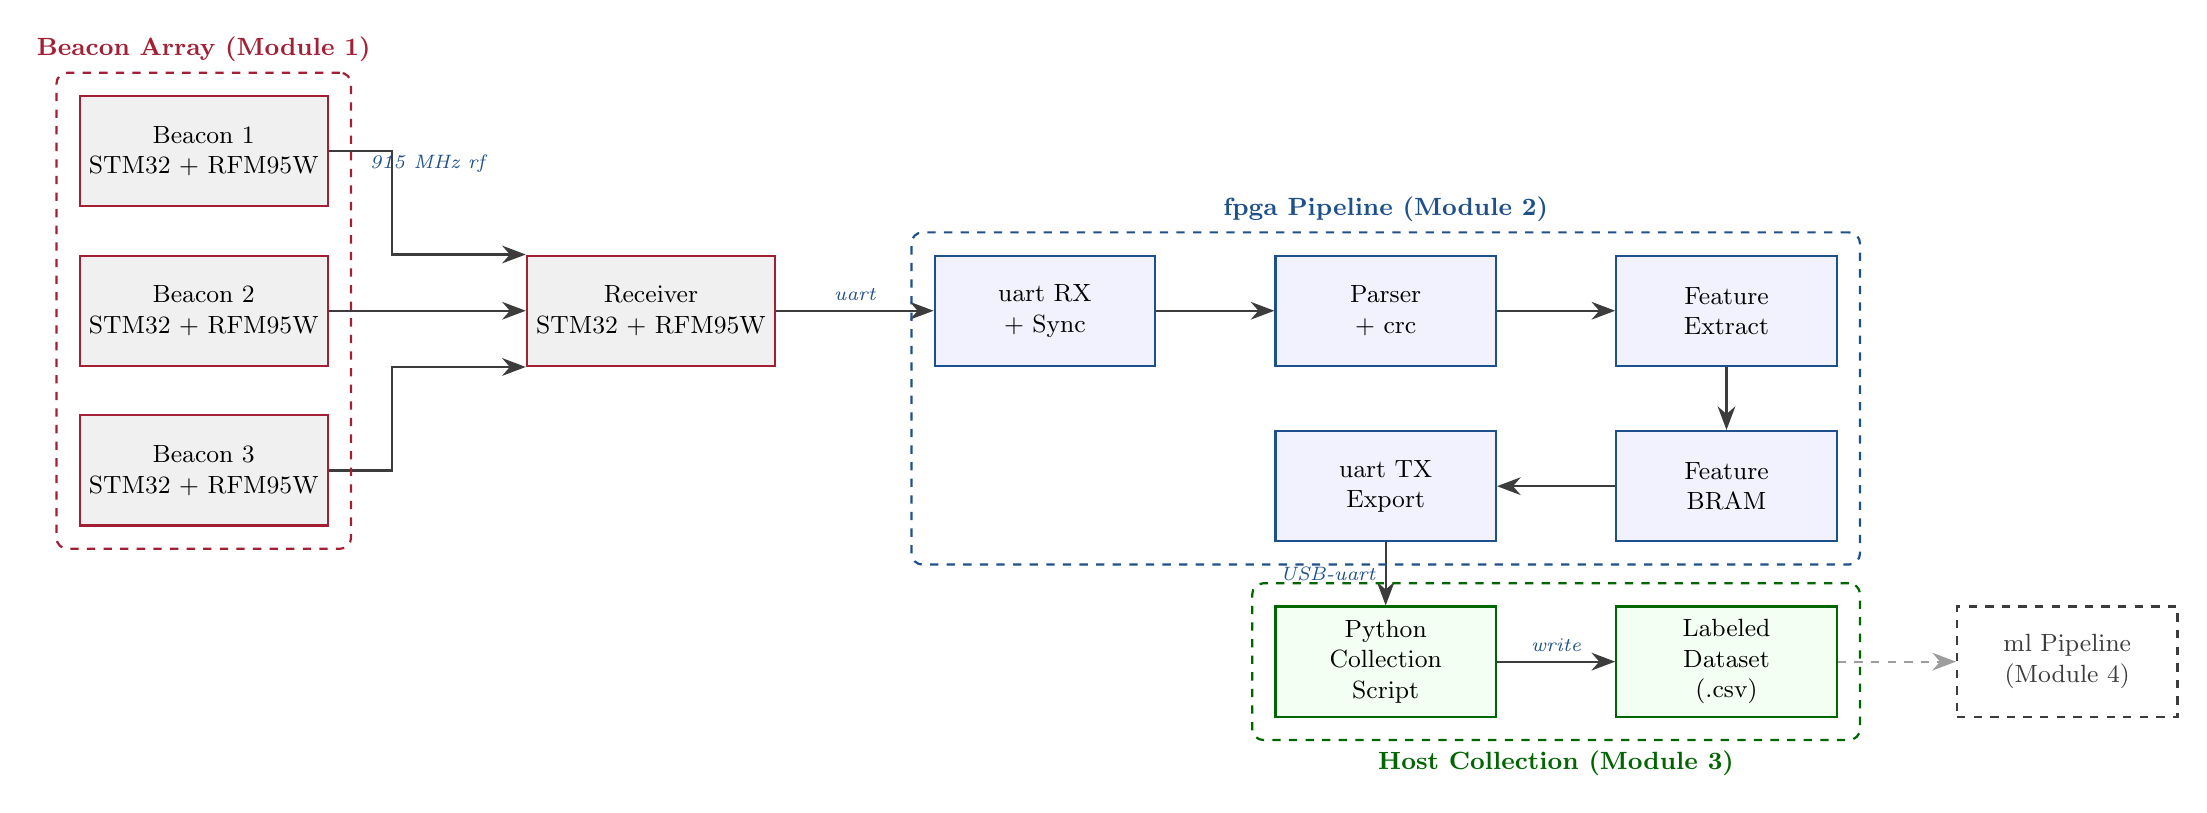
\begin{tikzpicture}[
				node distance=1.2cm and 1.8cm,
				hw/.style={rectangle, draw=stevens, fill=lightgray, thick,
					minimum width=2.8cm, minimum height=1.4cm, align=center, font=\small},
				fpga/.style={rectangle, draw=accentblue, fill=blue!5, thick,
					minimum width=2.8cm, minimum height=1.4cm, align=center, font=\small},
				sw/.style={rectangle, draw=green!40!black, fill=green!5, thick,
					minimum width=2.8cm, minimum height=1.4cm, align=center, font=\small},
				future/.style={rectangle, draw=darkgray, fill=white, thick, dashed,
					minimum width=2.8cm, minimum height=1.4cm, align=center, font=\small\color{darkgray}},
				arrow/.style={-{Stealth[length=3mm]}, thick, color=darkgray},
				elabel/.style={font=\scriptsize\itshape, color=accentblue}
				]

				% Beacons
				\node[hw] (b1) {Beacon 1\\STM32 + RFM95W};
				\node[hw, below=0.6cm of b1] (b2) {Beacon 2\\STM32 + RFM95W};
				\node[hw, below=0.6cm of b2] (b3) {Beacon 3\\STM32 + RFM95W};

				% Receiver
				\node[hw, right=2.5cm of b2] (rx) {Receiver\\STM32 + RFM95W};

				% \FPGA{} internals
				\node[fpga, right=2cm of rx] (uart_rx) {\UART{} RX\\+ Sync};
				\node[fpga, right=1.5cm of uart_rx] (parser) {Parser\\+ \CRC{}};
				\node[fpga, right=1.5cm of parser] (feat) {Feature\\Extract};
				\node[fpga, below=0.8cm of feat] (bram) {Feature\\BRAM};
				\node[fpga, below=0.8cm of parser] (uart_tx) {\UART{} TX\\Export};

				% Host
				\node[sw, below=0.8cm of uart_tx] (script) {Python\\Collection\\Script};
				\node[sw, right=1.5cm of script] (csv) {Labeled\\Dataset\\(.csv)};

				% Future
				\node[future, right=1.5cm of csv] (ml) {\ML{} Pipeline\\(Module 4)};

				% \RF{} arrows
				\draw[arrow] (b1.east) -- ++(0.8,0) |- (rx.north west);
				\draw[arrow] (b2.east) -- (rx.west);
				\draw[arrow] (b3.east) -- ++(0.8,0) |- (rx.south west);

				% Pipeline arrows
				\draw[arrow] (rx.east) -- (uart_rx.west) node[midway, above, elabel] {\UART{}};
				\draw[arrow] (uart_rx) -- (parser);
				\draw[arrow] (parser) -- (feat);
				\draw[arrow] (feat) -- (bram);
				\draw[arrow] (bram) -- (uart_tx);
				\draw[arrow] (uart_tx) -- (script) node[midway, left, elabel] {USB-\UART{}};
				\draw[arrow] (script) -- (csv) node[midway, above, elabel] {write};
				\draw[arrow, dashed, color=darkgray!50] (csv) -- (ml);

				% \RF{} label
				\node[font=\scriptsize\itshape, color=accentblue] at ($(b1.east)!0.5!(rx.north west)+(0,0.5)$) {915~MHz \RF{}};

				% Grouping boxes
				\node[draw=stevens, dashed, thick, rounded corners,
				fit=(b1)(b2)(b3),
				inner sep=8pt,
				label={[font=\small\bfseries\color{stevens}]above:Beacon Array (Module 1)}] {};

				\node[draw=accentblue, dashed, thick, rounded corners,
				fit=(uart_rx)(parser)(feat)(bram)(uart_tx),
				inner sep=8pt,
				label={[font=\small\bfseries\color{accentblue}]above:\FPGA{} Pipeline (Module 2)}] {};

				\node[draw=green!40!black, dashed, thick, rounded corners,
				fit=(script)(csv),
				inner sep=8pt,
				label={[font=\small\bfseries\color{green!40!black}]below:Host Collection (Module 3)}] {};
			\end{tikzpicture}%
		}
		\caption{Complete integrated system architecture at the end of Module~3. All connections are physical hardware interfaces validated end-to-end. The labeled dataset (green) is the primary output of this module and the input to Module~4.}
		\label{fig:full_system}
	\end{figure}

	\newpage
	% ══════════════════════════════════════════════════════════════
	\section{Hardware and Software Reference}
	\label{sec:hw_sw}
	% ══════════════════════════════════════════════════════════════

	\begin{table}[ht!]
		\centering
		\caption{Required hardware and software for Module 3.}
		\label{tab:hw_sw}
		\renewcommand{\arraystretch}{1.3}
		\begin{tabularx}{\textwidth}{l l X}
			\toprule
			\textbf{Item} & \textbf{Qty / Version} & \textbf{Purpose} \\
			\midrule
			STM32 Nucleo-L476RG & $\geq 3$ & 2 beacon MCUs + 1 receiver \MCU{} \\
			\RF{} Transceiver Module (RFM95W) & $\geq 3$ & Beacon and receiver \RF{} communication \\
			915~MHz Whip Antenna & $\geq 3$ & \RF{} transmission/reception \\
			Digilent Nexys A7-100T & 1 & \FPGA{} processing platform \\
			USB Micro-B Cables & 4--5 & Power, programming, and \UART{} communication \\
			Breadboard + Jumper Wires & --- & Inter-board connections (\UART{}, GND) \\
			Logic Analyzer (optional) & 1 & \UART{} waveform analysis during debugging \\
			Tape Measure & 1 & Physical distance measurement for Campaign C4 \\
			\midrule
			AMD Vivado Design Suite & 2024.1+ & Bitstream generation and \ILA{} debugging \\
			VS Code + STM32 extension stack & Latest & Beacon/receiver firmware modification (Module~1 reference environment; standalone STM32CubeIDE also supported) \\
			Python 3.10+ & --- & Host-side collection script and EDA \\
			\texttt{pyserial} & $\geq$3.5 & \UART{} communication from Python \\
			\texttt{pandas} & $\geq$2.0 & Dataset manipulation and merging \\
			\texttt{matplotlib} + \texttt{seaborn} & --- & EDA visualizations \\
			Terminal Emulator & --- & \UART{} debug and monitoring \\
			\bottomrule
		\end{tabularx}
	\end{table}

	% ══════════════════════════════════════════════════════════════
	\section{Assessment Rubric}
	% ══════════════════════════════════════════════════════════════

	\begin{table}[ht!]
		\centering
		\caption{Module 3 assessment rubric.}
		\label{tab:rubric}
		\renewcommand{\arraystretch}{1.3}
		\begin{tabularx}{\textwidth}{X c c}
			\toprule
			\textbf{Assessment Item} & \textbf{Weight} & \textbf{Due} \\
			\midrule
			Integration Debug Report (checklist, issue log, \ILA{} captures, field comparison) & 20\% & Week 1 \\
			System Performance Characterization Report (\PER{}, latency, throughput, scaling) & 25\% & Week 2 \\
			Data Collection Campaign Report Part 1 (experimental design, script, C1/C2 results) & 25\% & Week 3 \\
			Dataset and Data Collection Report Part 2 (C3--C5, merged dataset, EDA, distribution shift, data dictionary) & 30\% & Week 4 \\
			\bottomrule
		\end{tabularx}
	\end{table}

	\newpage
	% ══════════════════════════════════════════════════════════════
	\section{Recommended Resources}
	% ══════════════════════════════════════════════════════════════

	\subsection{Datasheets and Technical References}

	\begin{enumerate}[leftmargin=2em]
		\item Semtech, ``SX1276/77/78/79 Datasheet,'' Rev.\ 7, 2020. (Register map for \RSSI{}, \SNR{}, and frequency error readback.)
		\item STMicroelectronics, ``STM32L476xx Reference Manual,'' RM0351, Rev.\ 9, 2023. (\UART{} peripheral timing, \DMA{} configuration.)
		\item Digilent, ``Nexys A7 Reference Manual,'' Rev.\ C, 2022. (PMOD pinout, USB-\UART{} bridge specifications.)
		\item Xilinx/AMD, ``Vivado Design Suite User Guide: Programming and Debugging,'' UG908, 2023. (\ILA{} configuration, trigger setup, waveform capture.)
	\end{enumerate}

	\subsection{Integration and Testing References}

	\begin{enumerate}[leftmargin=2em]
		\item P.\ P.\ Chu, \textit{\FPGA{} Prototyping by \VHDL{} Examples: Xilinx Artix-7 Edition}, 2nd ed., Wiley, 2017. (Chapter on hardware verification and \ILA{} usage.)
		\item J.\ W.\ Valvano, \textit{Embedded Systems: Real-Time Interfacing to ARM Cortex-M Microcontrollers}, 6th ed., 2023. (\UART{} debugging techniques, logic analyzer usage.)
	\end{enumerate}

	\subsection{Data Science and Machine Learning Preparation}

	\begin{enumerate}[leftmargin=2em]
		\item W.\ McKinney, \textit{Python for Data Analysis}, 3rd ed., O'Reilly, 2022. (pandas, data cleaning, exploratory data analysis.)
		\item A.\ G\'eron, \textit{Hands-On Machine Learning with Scikit-Learn, Keras, and TensorFlow}, 3rd ed., O'Reilly, 2022. (Chapter 2: dataset splitting, stratified sampling, data exploration.)
		\item PySerial Documentation. [Online]. Available: \url{https://pyserial.readthedocs.io/}
	\end{enumerate}

	\subsection{Application Notes}

	\begin{enumerate}[leftmargin=2em]
		\item Semtech AN1200.22, ``LoRa Modulation Basics.'' (On-air time calculation for different SF/BW configurations.)
		\item Semtech AN1200.13, ``SX1276/7/8 LoRa Modem Design Guide.'' (Link budget, sensitivity, and interference behavior.)
	\end{enumerate}

	\newpage
	% ══════════════════════════════════════════════════════════════
	\section{Transition to Module 4}
	% ══════════════════════════════════════════════════════════════

	Upon successful completion of Module~3, students will have:
	\begin{itemize}[leftmargin=2em]
		\item A fully integrated and validated end-to-end pipeline: beacon \RF{} transmission $\rightarrow$ STM32 reception $\rightarrow$ \FPGA{} ingestion and feature extraction $\rightarrow$ host-side data collection.
		\item Characterized system performance with quantified \PER{}, latency, throughput, and scaling behavior across multiple beacon configurations.
		\item Diagnosed and resolved real cross-domain integration failures, gaining direct experience with the interface problems that span firmware, hardware, and digital logic boundaries.
		\item A labeled \RF{} dataset of approximately 2{,}500--3{,}500 feature vectors spanning 5 experimental campaigns with controlled variation of TX power, spreading factor, modulation type, distance, and beacon count.
		\item A host-side Python collection script and dataset pipeline that can be re-run to collect additional data if needed.
		\item Exploratory data analysis documenting feature distributions, correlations, and class balance.
		\item A quantitative understanding of the distribution shift between simulation data and hardware-collected data.
	\end{itemize}

	Module~4 will consume this dataset directly. Students will preprocess the \FPGA{}-extracted features, train and evaluate classifiers for spreading factor detection, modulation classification, and emitter identification, and analyze how classification accuracy varies as a function of \SNR{}, beacon count, and physical distance. The dataset's controlled experimental structure (single-variable sweeps with known ground truth) enables students to isolate which features drive model performance and which real-world factors degrade accuracy compared to simulation---questions that can only be answered with the kind of carefully collected, labeled hardware data this module produces.

	The distribution shift analysis from this module's EDA provides the empirical foundation for a key Module~4 experiment: training a classifier on simulation data (from the engagement simulator) and evaluating it on hardware data (from this module), then observing the accuracy drop as a direct measurement of the sim-to-real gap. This experiment is only possible because the framework stages data collection \emph{before} \ML{} development, giving students both data sources to compare.

	\vfill
	\clearpage
	\printnoidxglossary[type=\acronymtype,title={Glossary}]

	\begin{center}
		\rule{0.5\textwidth}{0.4pt}\\[6pt]
		{\small\textcolor{darkgray}{End of Module 3 Lesson Plan}}
	\end{center}

\end{document}
